% Kap E
\chapter{Das Jones-Polynom}

\Timestamp{2015-06-29}

% §E1
\section{Die Kaufman-Klammer und das Jones-Polynom}


Wir betrachten die Menge $\scr D^{\text{un}}$ der unorientierten Verschlingungsdiagramme (Nummerierung der Komponenten auch irrelevant).

\begin{prop}
    Sei $R$ ein kommutativer Ring mit 1 und $A, B, C \in R$.
    Dann gibt es genau eine Abbildung: $\<\argdot\> : \scr D^{\text{un}} \to R$, sodass gilt
    \begin{enumerate}[1)]
        \item
            $\<O\> = 1$, $\<D \sqcup O\> = \< D \> \cdot C$
            Insbesondere $\<O \dotso O\> = C^{n-1}$.
        \item
            $\<L_+\> = A \< L_1 \> + B \< L_2 \>$
    \end{enumerate}
    \begin{proof}
        \begin{seg}{Eindeutigkeit}
            Seien $\<\argdot\>, [\argdot]: \scr D^{\text{un}} \to R$ zwei Abbildungen mit den geforderten Eigenschaften.
            Induktion über die Kreuzungszahl $\Cr(D)$:
            Für $\Cr(D) = 0$ ist $\<D\> = C^{n-1} = [D]$ dank 1).
            Für $\Cr(D) \ge 1$ ist
            \begin{math}
                \< D L_+ \>
                = A \< L_1 \> + B \< L_2 \>
                = A [ L_1 ] + B [ L_2 ]
                = [D L_+ ].
            \end{math}
        \end{seg}
        \begin{seg}{Existenz}
            Rekursive Konstruktion von $\<\argdot\>: \scr D^{\text{num}} \to R$ (nummerierte Kreuzungen).
            Für $n = 0$:
            \begin{math}
                \< D \> := C^{\#D - 1}.
            \end{math}
            Für $n = 1$:
            \begin{math}
                \< D L_+ \> := A \< L_1 \> + B \< L_2 \>
            \end{math}
            Für $n = 2$:
            \begin{math}
                \< D L_+^1 L_+^2 \>
                &= A \< L_1 L_+ \> + B \< L_2 L_+ \> \\
                &= AA \< L_1 L_1\> + AB \< L_1 L_2 \> + BA \<L_2 L_1\> + BB \< L_2 L_2\> \\
                &= A \< L_+ L_2\> + B \< L_+ L_2\> \\
                &= \< D L_+^2 L_+^1 \>
            \end{math}
            Also ist $\< \argdot\>$ unabhängig von der Nummerierung der Kreuzungen.
            Wir erhalten $\< \argdot \>: \scr D \to R$.
        \end{seg}
    \end{proof}
\end{prop}

Reidemeister-Züge:
Wir erhalten für den R2-Zug die Bedingungen
\begin{math}
    B &= A^{-1}, &&
    C &= -A^2 - A^{-2}
\end{math}
Der R3-Zug ist damit bereits bedient.
Für den R1-Zug erhalten wir jedoch
\begin{math}
    \<K\> = (-A^{-3}) \<L\>
\end{math}
Wie erreichen wir Invarianz unter R1?
Brutale Methode: $-A^{-3} = 1$ algebraisch im Ring erzwingen.

Geschickter: Wir betrachten orientierte Diagramme und den Drall (w?) $w: \scr D^{\text{or}} \to \Z$, $w(D) = \sum_{p \text{ Kreuz}} \eps(p)$.
Der Drall ist invariant unter R2 und R3, aber $w(K) = w(L) + 1$.

\begin{df}
    Für jedes \emph{orientierte} Diagramm $D$ definieren wir das \emphdef{Jones-Polynom}
    \begin{math}
        V(D) = \<D\> \cdot (-A^{-3})^{w(D)}.
    \end{math}
    Dieses ist invariant unter allen R-Zügen.
    \begin{proof}
        Man betrachte den kritischen R1-Zug: Leicht.
    \end{proof}
\end{df}

\begin{st}
    Das Jones-Polynom definiert eine Abbildung $V: \scr L \to \Z[A^{\pm 1}]$.
\end{st}

\begin{ex}
    Für die Kleeblattschlinge erhalten wir
    \begin{math}
        V(3_1^-) = A^4 + A^{12} - A^{16}.
    \end{math}
\end{ex}

\begin{prop}
    Für $L \in \scr L$ gilt $V(L^!) = V(L)$

    Kehrt man die Orientierung von $L_1 \subset L$ um und lässt $L_2 = L \setminus L_1$ unverändert, dann gilt
    \begin{math}
        V(L_1^! \cup L_2)
        = V(L_1 \cup L_2) A^{6 \lk(L_1, L_2)}.
    \end{math}
\end{prop}

\begin{prop}
    Es gilt $V(L^*) = V(L)^*$, wobei $*: \Z[A^{\pm}] \to \Z[A^\pm]$ mit $A \mapsto A^{-1}$.
    \begin{proof}
        Stelle $L$ durch ein Diagramm $D$ dar.
        Die Aussage folgt induktiv aus
        \begin{math}
            w(D^*) &= -w(D) \\
            \<L_+\> &= A \< L_1\> + A^{-1} \<L_2\> \\
            \<L_-\> &= A^{-1} \< L_1\> + A \<L_2\>.
        \end{math}
        Alternativ mit Eindeutigkeit:
        \begin{math}
            [D] := \<D^*\>^*
        \end{math}
        erfüllt die Bedingung für die Kaufman-Klammer, also $[\argdot] = \<\argdot\>$.
    \end{proof}
\end{prop}

\begin{ex}
    \begin{math}
        V(3_1^-) &= A^4 + A^{12} - A^{16}, \\
        V(3_1^+) &= A^{-4} + A^{-12} - A^{-16}.
    \end{math}
    Das Jones-Polynom unterscheidet also links- und rechtshändige Kleeblattschlinge.
    Dies ist neben Färbungspolynom und Signatur unser dritter Beweis für die Chiralität der Kleeblattschlinge.
\end{ex}

\begin{prop}
    \begin{math}
        V(K \# L) = V(K) V(L)
    \end{math}
    (Vorsicht: linke Seite nur für Knoten wohldefiniert)
    \begin{proof}
        Stelle $K$, $L$ durch Diagramme dar, kurz: $D \# D'$.
        Induktion über $\Cr(D')$: für $\Cr(D') = 0$ ist alles klar.

        Siehe Skizze.
    \end{proof}
\end{prop}

\begin{nt}
    Übliche Schreibweisen für das Polynom $V(K)$: in den Variablen $q = -A^{-2}$, bzw. $t = A^{-4} = q^2$.
\end{nt}

\begin{st}
    Die Invariante $V: \scr D^{or} \to \Z[q^\pm 1] \subset \Z[A^{\pm 1}]$ erfüllt $V(0) = 1$ und die Schienenrelation
    \begin{math}
        q^{-2} V(L_+) - q^2 V(L_-) = (q^{-1} - q^{+1}) V(L_0).
    \end{math}
    Dies legt $V$ eindeutig fest und liefert zugleich einen Algorithmus.
    \begin{proof}
        \begin{math}
            A \<L_+\> &= A^2\<L_1\> + A^0 \< L_2\> \\
            A^{-1} \<L_-\> &= A^{-2}\< L_1\> + A^0 \< L_2 \> \\
            \leadsto q^{-2}V(L_+) - q^2 V(L_-) &= A^4 (-A^{-3})^{w+1} \< L_+\> - A^{-4} (-A^{-3})^{w-1} \<L_-\> \\
            &= (-A^{-3})^w \Big( -A \<L_+\> + A^{-1} \<L_-\> \Big) \\
            &= (-A^{-3})^w (A^{-2} - A^2) \< L_2 \> \\
            &= (q^{-1} - q) V(L_0)
        \end{math}
    \end{proof}
    \begin{nt}
        Das Alexander-Polynom hatte die Eigenschaft $\Delta(0) = 1$,
        \begin{math}
            \Delta(L_+) - \Delta(L_-) = (q-q^{-1}) \Delta(L_0).
        \end{math}
        Die Determinante: $\det(0) = 1$,
        \begin{math}
            \det(L_+) - \det(L_-) = 2i \det(L_0).
        \end{math}
        Es gilt
        \begin{math}
            \det = \Delta|_{q\mapsto i}
            = V|_{q \mapsto i}.
        \end{math}
    \end{nt}
\end{st}

\Timestamp{2015-07-01}

Für das Jones-Polynom gibt es zwei Zugänge
\begin{enumerate}[1)]
    \item
        Kaufmann-Klammer, $\<D\> \in \Z[A^{\pm 1}]$, Drall-Normierung $V(D) = \<D\> (-A^{-3})^{w(D)}$.
    \item
        Schienenrelation:
        \begin{math}
            q^{-2} V(L_+) - q^2 V(L_-) = (q^{-1} - q) V(L_0)
        \end{math}
        übliche Konvention: $q := -A^{-2}$, bzw $t = A^{-4} = q^2$.
\end{enumerate}
1) hatten wir bereits behandelt.
2) lässt sich auch als Konstruktion für das Jones-Polynom verwenden.

Vergleiche das Alexander-Polynom: $\Delta: \scr L \to \Z[q]$:
\begin{math}
    \Delta(L_+) - \Delta(L_-) = (q-q^{-1}) \Delta(L_0).
\end{math}
\begin{note}
    $V$ unterscheidet viele Knoten, die $\Delta$ nicht unterscheidet, z.B. $3_1 \neq 3_1^x$.
    Umgekehrt gibt es Knoten $K, L$ mit $\Delta(K) \neq \Delta(L)$, aber $V(K) = V(L)$.
    Beide Invarianten sind also unabhängig.
\end{note}
Ein Defekt, oder eine Eigenschaft beider Polynome ist die Invarianz unter Mutation (Drehung einer passenden Komponente um 180 Grad):

\begin{ex}
    Conway-Knoten $C$ und Kinoshita-Terasaka-Knoten $K$.
\end{ex}

\begin{st}
    Sei $I: \scr D^{\text{or}} \to R$, $a,b,c \in R$, $a,b \in \R^*$ eine Invariante mit $I(0) = 1$ und
    \begin{math}
        a I(L_+) + b I(L_-) = c I(L_0).
    \end{math}
    Dann ist $I$ invariant unter Mutation.
    \begin{proof}
        Induktion über $\Cr(R)$.
        Für $\Cr(R) = 0$ ist dies klar (2 Fälle mit evtl. Kreiskomponenten, die beliebig verschoben werden können).
        Sei nun $\Cr(R) \ge 1$.
        Mache Strang 1 absteigend, dann 2.
        Wenn absteigend, dann klar: (4 Fälle).

        Nun Induktion über die Anzahl $n$ der zu wechselnden Kreuzungen bis absteigend ($n=0$ trivial).
        Es gilt
        \begin{math}
            \text{Skizze}
        \end{math}
    \end{proof}
\end{st}

\begin{ex}
    Für Conway-Knoten und K-T-Knoten $K$ gilt $\Delta(C) = \Delta(K)$, $V(C) = V(K)$.
    Wie unterscheidet man also $K$ und $C$?
    Es geht mit Färbungspolynomen, z.B. mit $G = \PSL_2 \F_7$, $x = \Matrix{0 & 1 \\ -1 & 1}$, $\od(x) = 3$.
    Es ergibt sich
    \begin{math}
        P_G^x(K) &= 1 + 6x, &&
        P_G^x(C) &= 1 + 12x.
    \end{math}
    Ebenso mit $G = A_7$, $x = (1234567)$,
    \begin{math}
        P_G^x(K) &= 1 + 7x^2 + 28x^5 + 18x^6 \\
        P_G^x(C) &= 1 + 7x^2 + 7x^3 + 21x^5 + 14x^6
    \end{math}
    Mit $G = M_{11} \subset A_{11}$ findet man sogar $K \neq K^x, K^!, K^*$ und $C \neq C^x, C^!, C^*$.
\end{ex}

\begin{nt}
    Die Berechnung des Alexander-Polynoms $\Delta$ ist relativ leicht und effizient (dank linearer Algebra).
    Die Berechnung von $V$ ist aufwändiger.
    Nur wenige spezielle Werte lassen sich anders und schneller berechnen.
\end{nt}

\begin{prop}
    \begin{enumerate}[1)]
        \item
            $V(L)|_{q\mapsto 1} = 2^{\# L - 1}$,
        \item
            $V(L)|_{q\mapsto i} = \det(L)$,
        \item
            $V(L)|_{q\mapsto e^{\frac{\pi i}{6}}} = \pm (i\sqrt{3})^{\Col_3(L)}$
    \end{enumerate}
    \begin{proof}
        \begin{enumerate}[1)]
            \item
                Induktion per Schienenrelation
            \item
                Induktion per Schienenrelation
            \item
                vermutlich nicht-trivial.
        \end{enumerate}
    \end{proof}
\end{prop}

\begin{nt}
    Für den Torusknoten $T(a,b)$ kennt man geschlossene Formeln für $\Delta$ und $V$.
    Im Allgemeinen bleibt es bei mühsamen Rechnungen für Einzelfälle.
\end{nt}


% §E2
\section{Verallgemeinerungen zum HOMFLYPT-Polynom und zum Kauffman-Polynom}

\begin{lem}
    Zu $D \in \scr D_n^*$ ist das absteigende Diagramm $\alpha D$ trivial.
    Genauer existiert eine Folge von R-Zügen
    \begin{math}
        \alpha D = D_0 \to D_1 \to \dotsb \to D_l = 0
    \end{math}
    mit der Eigenschaft, dass $\Cr(D_0) \ge \Cr(D_1) \ge \dotsb \ge \Cr(D_l) = 0$.
    Hierbei erlauben wir neben $R1, R2, R3$ auch $R2^2$ (zweifache Anwendung von R2, durchschieben von einem Kreis).
    \begin{proof}
        Übung, oder Lickorisk Kap 15.
    \end{proof}
    \begin{note}
        Ohne $R2^2$ ist dies nicht möglich (Skizze: 8 mit zwei zusätzlichen inneren Komponenten).
    \end{note}
\end{lem}

\begin{st}[HOMPFLYPT]
    Sei $R$ ein kommutativer Ring mit Eins, $a, b \in R^*$, $c, d \in R$ mit $a - b = cd$.
    Dann existiert genau eine Abbildung $I: \scr D^{\text{or}} \to R$ mit
    \begin{enumerate}[i)]
        \item
            $I(0) = 1$ und $I(D \sqcup 0) = I(D) \cdot d$,
        \item
            $aI(L_+) - bI(L_-) = cI(L_0)$,
        \item
            $I$ ist invariant unter Reidemeister-Zügen.
    \end{enumerate}
    \begin{proof}
        Die Eindeutigkeit wurde bereits bewiesen (durch Algorithmus).
        Die Existenz verlangt nach einer Konstruktion.

        Sei $\scr D_n$ die Menge der Verschlingungsdiagrammen mit $\le n$ Kreuzungen.
        Sei $\scr D_n^*$ die Menge der Verschlingungsdiagrammen mit $\le n$ Kreuzungen und nummerierten Komponenten mit jeweils einem Basispunkt auf der Komponente.

        Zu einem Diagramm $D \in \scr D_n^*$ ist das absteigende Diagramm $\alpha D$ eindeutig bestimmt (Komponenten jeweils von Basispunkt absteigend).

        Konstruktion von $I_n: \scr D_n^* \to R$ und Nachweis der Eigenschaften:
        \begin{seg}{$n = 0$}
            $I_0: \scr D_0^* \to R$, setze $I_0(D) = d^{\#D - 1}$ ($d$ Anzahl der Komponenten).
        \end{seg}
        \begin{seg}{$n \ge 1$}
            Sei $I_{n-1}$ konstruiert.
            Definiere $I_n$ wie folgt.
            Sei $w(D)$ die Anzahl der zu wechselnden Kreuzungen von $D$ nach $\alpha D$.
            Für $w(D) = 0$ setze $I_n(D) = d^{\#D - 1}$ gemäß 1).
            Für $w(D) \ge 1$ wechsle die erste Kreuzung und berechne $I_n(D)$ gemäß 2).
        \end{seg}
        Wir zeigen
        \begin{enumerate}[($A_n$)]
            \item
                $I_n(D)$ ist unabhängig von der Reihenfolge der zu wechselnden Kreuzungen.
            \item
                $I_n(D)$ ist unabhängig von den Basispunkten.
            \item
                $I_n(D)$ ist invariant unter Reidemeister-Zügen in $\scr D_n^*$ (solche, die die Kreuzungszahl nicht ändern).
            \item
                $I_n(D)$ ist unabhängig von der Nummerierung der Komponenten.
        \end{enumerate}
        $A_0, B_0, C_0, D_0$ sind klar.
        Seien $A_{n-1}, B_{n-1}, C_{n-1}, D_{n-1}$ bewiesen.
        \begin{seg}{$A_n$: Reihenfolge der zu wechselnden Kreuzungen}
            $A_n$ gilt dank Kommutativität:
            \begin{math}
                a I_n(L_+ L_+) - b I_n(L_- L_+) &= c I_{n-1}(L_0 L_+) \\
                a I_n(L_- L_+) - b I_n(L_- L_-) &= c I_{n-1}(L_- L_0) \\
                \leadsto
                a^2 I_n(L_+ L_+) - b^2 I_n(L_- L_-) &= ac I_{n-1}(L_0 L_+) + bc I_{n-1}(L_- L_0)
            \end{math}
            und
            \begin{math}
                a I_n(L_+ L_+) - b I_n(L_+ L_-) &= c I_{n-1}(L_+ L_0) \\
                a I_n(L_+ L_-) - b I_n(L_- L_-) &= c I_{n-1}(L_0 L_-) \\
                \leadsto
                a^2 I_n(L_+ L_+) - b^2 I_n(L_- L_-) &= ac I_{n-1}(L_+ L_0) + bc I_{n-1}(L_0 L_-)
            \end{math}
            Die Differenz ist
            \begin{math}
                c^2 I_n(L_0 L_0) - c^2 I_n(L_0 L_0) &= 0
            \end{math}
            Damit gilt $A_n$, d.h. $I_n$ erfüllt die Schienenrelation 2) für jede Kreuzung.
        \end{seg}
\Timestamp{2015-07-06}
        \begin{seg}{$B_n$: Verschiebung eines Startpunktes}
            Überqueren einer Kreuzung $D \leadsto D'$ von Komponente $i$ über Komponente $j$.
            Für $i \neq j$ ist $\alpha D = \alpha D'$ und $I_n(D) = I_n(D')$.
            Für $i = j$ unterscheiden sich $\alpha D$ und $\alpha D'$ nur durch einen Kreuzungswechsel.
            Unter Verwendung von $A_n$ ist die Reihenfolge der Krezungen nicht relevant.
            %\begin{math}
            %    I_n(D) - I_n(\alpha D) = d^{\#D-1}
            %    I_n(D') - I_n(\alpha D') = d^{\#D-1}
            %\end{math}
            Induktiv:
            \begin{math}
                a I_n(L_+) - b I_n(L_-) &= c I_{n-1}(L_0) \\
                a I_n(L_+) - b d^{\# D - 1}&= c d^{\#D_0 - 1} = (a-b)d^{\#D -1} \\
            \end{math}
            Es folgt $I_n(L_+) = d^{\# D - 1}$.
        \end{seg}
        \begin{seg}{$C_n$: Reidemeisterzüge}~\vspace{-1em}
            \begin{enumerate}[(R1)]
                \item
                    Induktion über Anzahl $w(D)$ der zu wechselnden Kreuzungen von $D$ nach $\alpha D$.
                    Nach entsprechender Verschiebung von $*$ gilt $w(D) = w(D')$.
                    Für $w(D) = w(D') = 0$ ist alles klar.
                    \begin{math}
                        I_n(D) = d^{\# D - 1} = d^{\# D' - 1} = I_n(D).
                    \end{math}
                    Sei $w(D) = 1$.
                    Dann wechsle eine Kreuzung:
                    \begin{math}
                        a I_n(R L_+) - b I_n(R L_-) &= c I_{n-1}(R L_0) \\
                        a I_n(R' L_+) - b I_n(R' L_-) &= c I_{n-1}(R' L_0)
                    \end{math}
                    Rechte Seiten sind gleich dank $C_{n-1}$, die zwei Terme auf den linken Seiten ebenfalls dank Induktion über $w(D)$.
                \item
                    Für Komponenten $i = j$ einfach durch entsprechende Verschiebung des Startpunktes und Induktion wie oben.
                    Betrachte $i \neq j$: unterscheide $i < j$ und $i > j$, ein Fall ist einfach, sonst Wechsel der Kreuzungen:
                    Ausrechnen ergibt
                    \begin{math}
                        a I_n(R_{-+}) - b I_n(R_{--}) &= c I_{n-1}(R_{-0}) \\
                        a I_n(R_{+-}) - b I_n(R_{--}) &= c I_{n-1}(R_{0-})
                    \end{math}
                    und folglich $I_n(R_{-+}) = I_n(R_{+-})$.
                    Ebenso mit anderer Orientierung (Übung).
                \item
                    \begin{math}
                        a I_n(R_{**,+}) - b I_n(R_{**,-}) &= I_{n-1}(R_{**,0}) \\
                        a I_n(R_{+,**}) - b I_n(R_{-,**}) &= I_{n-1}(R_{0,**})
                    \end{math}
                    Die rechten Seiten sind gleich.
                    Diskussion aller Fälle:
                    Der Fall $i < j < k$ ist einfach mit $\impliedby$, ebenso $i < k < j$ mit $\implies$.
                    Sei nun $k < j < i$, wir wechseln die Kreuzungen $ij, ik$, um auf einen bekannten Fall zurückzuführen.
                    Erste Orientierung von $i$:
                    Der bekannte Fall wäre $I_n(R_{++,+}) = I_n(R_{+,++})$.
                    Zu zeigen: $I_n(R_{--,+}) = I_n(R_{++,+})$.
                    \begin{math}
                        a I_n( R_{-+,+}) - b I_n(R_{--,+}) &= c I_{n-1}( R_{-+,+} ) \\
                        a I_n( R_{++,+}) - b I_n(R_{-+,+}) &= c I_{n-1}( R_{0+,+} ) \\
                        a I_n( R_{+,+-}) - b I_n(R_{+,--}) &= c I_{n-1}( R_{+,0-} ) \\
                        a I_n( R_{+,++}) - b I_n(R_{+,+-}) &= c I_{n-1}( R_{+,+0} ) \\
                    \end{math}
                    Nun ergibt sich
                    \begin{math}
                        a^2 I_n( R_{++,+}) - b^2 I_n(R_{--,+}) &= b c I_{n-1}(R_{-0,+}) + ac I_{n-1}(R_{0+,+}) \\
                        a^2 I_n( R_{+,++}) - b^2 I_n(R_{+,--}) &= b c I_{n-1}(R_{+,0-}) + ac I_{n-1}(R_{+,+0}) \\
                    \end{math}
                    Dank R2 ist $I_n(R_{-0,+}) = I_n(R_{+,0-})$.
                    Auf der linken Seite ergeben sich eine Äquivalenz, mit der wir alle Stränge permutieren können.
                    Für eine Permutation ist die R3-Invarianz klar, damit auch für alle anderen.

                    Ebenso für die zweite Orientierung von $i$:
                    Auch $i = j < k$ und andere Fälle verlaufen analog oder leichter.
                \item[$R2^2$]
                    klar, nichts zu zeigen.
            \end{enumerate}
        \end{seg}
        \begin{seg}{$D_n$: Unabhängig von Nummerierung}
            Sei $D \leadsto D'$ ein Umnummerierung.
            Induktion über $w(D)$.
            Für $w(D) = 0$ erhält man dank Reidemeister-Züge (monoton fallend in $\scr D_n^*$) disjunkte Kreise.
            $C_n$ liefert also $I_n(D') = d^{\# D - 1} = I_n(D)$.
            Für $w(D) \ge 1$ wechsle eine Kreuzung und schließe per Induktion.
        \end{seg}
    \end{proof}
\end{st}

\Timestamp{2015-07-08}

\begin{ex}
    \begin{itemize}
        \item
            Alexander-Polynom: $R = \Z[q^\pm]$ und
            \begin{math}
                a &= b = 1, &&
                c &= q - q^{-1}, &&
                d &= 0.
            \end{math}
        \item
            Alexander-Conway: $R = \Z[z]$ und
            \begin{math}
                a &= b = 1, &&
                c &= z, &&
                d &= 0.
            \end{math}
        \item
            Jones-Polynom: $R = \Z[q^\pm]$ und
            \begin{math}
                a &= q^{-2}, &&
                b &= q^2, &&
                c &= q^{-1} - q, &&
                d &= q^{-1} + q.
            \end{math}
        \item
            HOMFLYPT-Polynom: $R = \Z[l^\pm, m, \frac{l^{-1} - l}{m}] \subset \Z[l^\pm, m^\pm]$ und
            \begin{math}
                a &= l^{-1}, \\
                b &= l, \\
                c &= m, \\
                d &= \frac{l^{-1} - l}{m}.
            \end{math}
            Spezialisieren mit $(l, m) \mapsto (1, q - q^{-1})$ liefert das Alexander-Polynom.
            Spezialisieren mit $(l, m) \mapsto (q^2, q^{-1} - q)$ liefert das Jones-Polynom.

            Spezialisieren mit $(l, m) \mapsto (q^n, q^{-1} - q)$ liefert
            \begin{math}
                d
                = \frac{l^{-1} - l}{m}
                = \frac{q^{-n} - q^n}{q^{-1} - q}
                = q^{1-n} + q^{3-n} + \dotsb + q^{n-3} + q^{n-1}.
            \end{math}
            Hier liefert $n = 1$ eine triviale Invariante (Warum? Übung).
    \end{itemize}
\end{ex}

Ebenso beweist man:

\begin{st}[Kauffman, 1990]
    Es existiert genau eine Abbildung $\Lambda: \scr D^{\text{un}} \to \Z[a^\pm, z^\pm]$ mit
    \begin{enumerate}[i)]
        \item
            $\Lambda(0) = 1$, $\Lambda(R1^*) = a \Lambda(R1^0)$,
        \item
            $\Lambda(L_+) + \Lambda(L_-) = z\Big(\Lambda(L_|) + \Lambda(L_-)\Big)$,
            (beachte: keine Orientierung)
        \item
            $\Lambda$ ist invariant unter R2/3-Zügen.
    \end{enumerate}
    Die Abbildung $F: \scr D^{\text{or}} \to \Z[a^\pm, z^\pm]$ mit $F(D) = a^{-w(D)} \Lambda(D)$ ist invariant unter R1/2/3-Zügen.
\end{st}


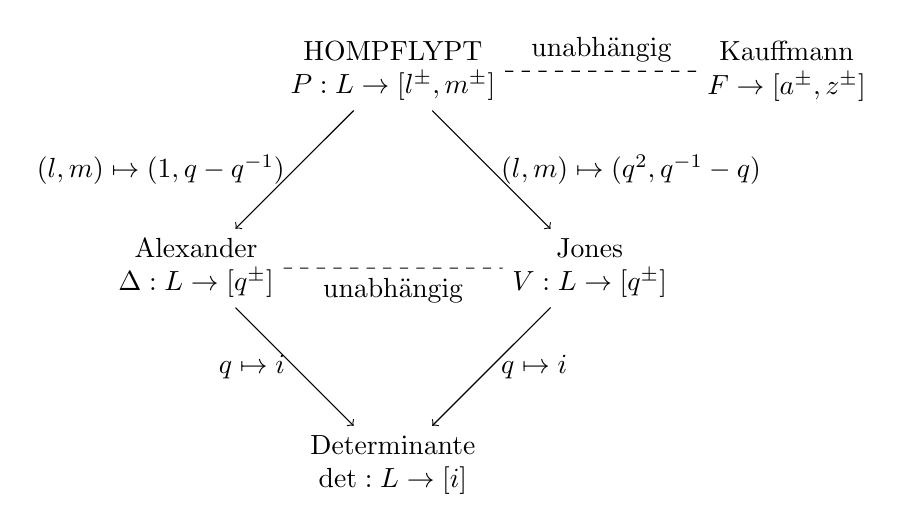
\begin{tikzpicture}[scale=2.5]
    \node[align=center] (1) at (1,2) {HOMPFLYPT \\ $P: \scr L \to \Z[l^\pm, m^\pm]$};
    \node[align=center] (2) at (0,1) {Alexander \\ $\Delta: \scr L \to \Z[q^\pm]$};
    \node[align=center] (3) at (2,1) {Jones \\ $V: \scr L \to \Z[q^\pm]$};
    \node[align=center] (4) at (1,0) {Determinante \\ $\det: \scr L \to \Z[i]$};
    \node[align=center] (5) at (3,2) {Kauffmann \\ $\scr F \to \Z[a^\pm, z^\pm]$};

    \draw[->] (1) -- node[left] {$(l,m) \mapsto (1, q - q^{-1})$} (2);
    \draw[->] (1) -- node[right] {$(l,m) \mapsto (q^2, q^{-1} - q)$} (3);
    \draw[->] (2) -- node[left] {$q \mapsto i$} (4);
    \draw[->] (3) -- node[right] {$q \mapsto i$} (4);
    \draw[dashed] (1) -- node[above] {unabhängig} (5);
    \draw[dashed] (2) -- node[below] {unabhängig} (3);
\end{tikzpicture}


% §E3
\section{Die Tait-Vermutung}

\begin{df}
    Ein Verschlingungs-Diagramm $D \subset \R^2$ heißt \emphdef{alternierend}, wenn beim Durchlaufen jeder Komponente abwechselnd Über/Unterkreuzungen auftauchen.

    Eine Verschlingung $L \subset \R^3$ heißt \emphdef{alternierend}, wenn sie sich durch ein alternierendes Diagramm darstellen lässt.
\end{df}

\begin{nt}
    \begin{itemize}
        \item
            In alternierenden Diagrammen ist kein R3-Zug möglich (die entsprechenden Situation können nicht auftreten):
        \item
            Ebensowenig ist ein reduzierender R2-Zug möglich (nicht-reduzierend möglich).
        \item
            Reduzierende R1-Züge sind möglich.
        \item
            Allgemeiner ist folgendes möglich: (zwei Teile, eins umkehren, „großer R1-Zug“ siehe Skizze)
    \end{itemize}
\end{nt}

\begin{df}
    Ein Diagramm heißt \emphdef{reduziert}, wenn keine solche Reduktion mehr möglich ist.
\end{df}

Die drei Tait-Vermutungen besagen
\begin{enumerate}[(1)]
    \item
        Jedes reduzierte, alternierende Verschlingungsdiagramm $D$ minimiert die Kreuzungsszahl, d.h. $D' \sim D \implies \Cr(D') \ge \Cr(D)$.
    \item
        Für reduzierte, alternierende Diagramme $D$ ist der Drall $w(D) = \sum_{p} \eps(p)$ eine Invariante, d.h. $D' \sim D$ mit $D, D'$ reduziert und alternierend impliziert $w(D) = w(D')$.
    \item
        Sind $D \sim D'$ reduzierte alternierende Diagramme, dann lassen sie sich allein durch Flypes (in $\S^2$) ineinander überführen.
\end{enumerate}
\begin{note}
    Klar ist $(3) \implies (2)$.
\end{note}
Dies löst das Klassifikationsproblem für alternierende Verschlingungen.


\begin{df}
    Jedes Polynom $P \in \Z[A^\pm]$, $P \neq 0$ schreibt sich eindeutig als
    \begin{math}
        P = \sum_{k=m}^n p_k A^k
    \end{math}
    mit $p_m \neq 0 \neq p_n$, $m \le n$.
    Wir setzen $\mindeg(P) := m$ und $\maxdeg(P) := n$ und $\width(P) := n - m$.
\end{df}

\begin{ex}
    \begin{enumerate}[1.]
        \item
            Beim Alexander-Polynom war $\width_q(\Delta(D) \le 4g(S_D)$.
            Gleichheit gilt falls $D$ zusammenhängend und alternierend ist (ohne Beweis).
        \item
            Wir wollen dies für Jones und die Kreuzungszahl $\Cr$ zeigen.
    \end{enumerate}
\end{ex}

\begin{df}
    Sei $D \subset \R^2$ ein unorientiertes Diagramm mit nummerierten Kreuzungen $i = 1, \dotsc, n$.
    Zu $s: \Set{1, \dotsc, n} \to \Set{\pm 1}$ definiere ein „aufgelöstes“ Diagramm $sD$ durch
    \begin{math}
        …
    \end{math}
    Sei $|sD|$ die Anzahl der Kreise und $\sum s := \sum_{i=1}^n s(i)$ die Summe der Vorzeichen.
\end{df}

\begin{lem}
    Für die Kaufmann-Klammer gilt
    \begin{math}
        \<D\> &= \sum_{s: \Set{1, \dotsc, n} \to \Set{\pm 1}} A^{\sum s} (-A^2 - A^{-2})^{|sD|-1} \\
        &=: \sum_{s} \< D | s\>
    \end{math}
\end{lem}

Ziel: Für reduzierte alternierende Diagramme wollen wir $\width(\<D\>)$ berechnen, genauer: höchste und niedrigste Terme verstehen.


\Timestamp{2015-07-13}

Definition: Distante Vereinigung.

\begin{df}
    Ein Diagramm $D$ heißt \emphdef{zusammenhängend}, wenn es nicht distante Vereinigung ist, d.h. $D = D_1 \sqcup D_2$ folgt entweder $D_1 = \emptyset$ oder $D_2 = \emptyset$.

    Ausführlich: Sei $S^1 \homto \C \subset \R^2$ eine (polygonale) Jordan-Kuve und $\R^2 \setminus C = A \sqcup B$ zwei Gebiete.
    Wenn $C \cap D = \emptyset$, dann entweder $A \cap D = \emptyset$ oder $B \cup D = \emptyset$.
\end{df}

Definition: Verbunde Summe von Diagrammen $D = D_1 \# D_2$.

\begin{df}
    Ein Diagramm $D$ heißt \emphdef{prim}, wenn es nicht verbundene Summe ist, d.h. aus $D = D_1 \# D_2$ folgt entweder $D_1$ oder $D_2$ trivial (ohne Kreuzungen).

    Ausführlich: Besteht $C \cap D$ aus zwei transversalen Schnittpunkten, dann ist entweder $A \cap D$ oder $B \cap D$ trivial, d.h. ein Bogen ohne Kreuzungen.
\end{df}

Dies sind Eigenschaften des Diagramms, nicht der zugrundeliegenden Verschlingung (Beispiele: zwei Kreiskompenten übereinander, nebeneinander und zwei Kleeblattschlingen als verbundene Summe nebeneneinander und teilweise übereinander).

\begin{st}
    Sei $D \subset \R^2$ ein unorientiertes Diagramm.
    Durch Auflösen einer Kreuzung erhalten wir aus $D$ die Diagramme $D_-$ oder $D_+$ (je nachdem wie die Kreuzung aufgelöst wurde).
    \begin{enumerate}[a)]
        \item
            Ist $D$ zusammenhängend, so auch $D_+$ oder $D_-$ (oder beide).
        \item
            Ist $D$ prim, so auch $D_+$ oder $D_-$ (oder beide).
    \end{enumerate}
    \begin{proof}
        \begin{enumerate}[a)]
            \item
                Angenommen $D$ ist zusammenhängend, aber weder $D_+$ noch $D_-$.
                Die trennenden Jordankurven $C_+, C_-$ müssen durch die aufgelösten Kreuzungen gehen (nach geeignetem Umformen nur einmal).
                Der Rand des Innenbereichs von $C_+$ und $C_-$ schneidet $D$ genau ein Mal, ein Widerspruch.
            \item
                Angenommen $D$ ist prim, aber weder $D_+$ noch $D_-$.
                Im Gegensatz zu oben sind hier jeweils zwei Fälle für $C_+$ und $C_-$ zu unterscheiden (Schnitte außen oder innen).
                Beim Schneiden von $C_+$ und $C_-$ sind weitere Fälle zu unterscheiden.
                $C_+ \cup C_-$ zerlegt die Ebene in vier offene Mengen (mit jeweils evtl. mehreren Zusammenhangskomponenten)
                \begin{math}
                    AA &= \Set{z \in \R^2 & \deg(C_-,z) = 0, \deg(C_+,z) = 0} \\
                    AB &= \Set{z \in \R^2 & \deg(C_-,z) = 0, \deg(C_+,z) = 1} \\
                    BA &= \Set{z \in \R^2 & \deg(C_-,z) = 1, \deg(C_+,z) = 0} \\
                    BB &= \Set{z \in \R^2 & \deg(C_-,z) = 1, \deg(C_+,z) = 1}.
                \end{math}
                Aus Paritätsgründen haben genau zwei dieser Bereiche $E_1, E_2$ genau zwei Schnitte mit $D$.
                Diese zwei Bereiche können nicht $AA$ und $BB$ sein.
                $D$ muss ohne Einschrankung in $E_1$ Kreuzungen enthalten ($C_+, C_-$ waren nicht-triviale Zerlegungen von $D_+, D_-$).
                $E_1$ liefert dann eine nicht-triviale Zerlegung für $D$, ein Widerspruch.
        \end{enumerate}
    \end{proof}
\end{st}

Die erste Tait-Vermutung wird präzisiert und umfassend beantwortet durch den folgenden Satz.

\begin{st}
    Sei $D \subset \R^2$ ein zusammenhängendes Verschlingungsdiagramm und $L \subset \R^3$ die dargestellte Verschlingung mit Jones-Polynom $V(L) \in \Z[q^\pm]$.
    \begin{enumerate}[a)]
        \item
            Es gilt
            \begin{math}
                \frac{1}{2} \width_q V(L) \le \Cr(D)3
            \end{math}
        \item
            Gleichheit gilt, wenn $D$ reduziert alternierend ist oder verbundene Summe solcher Diagramme ist.
        \item
            In allen anderen Fällen ist die Ungleichung strikt, d.h. es wird keine Gleichheit angenommen.
    \end{enumerate}
\end{st}


\Timestamp{2015-07-15}

\begin{lem}[Umschalten von $+$ nach $-$]
    Seien $s, s': \Set{1, \dotsc, n} \to \Set{\pm 1}$ mit $s(i) = +1$, $s'(i) = - 1$ für ein $i$ und $s(j) = s'(j)$ für alle $j \neq i$.

    Dann gilt $\sum s' = \sum s - 2$ und $|s'D| = |sD| \pm 1$.
    \begin{proof}
        Löse eine Kreuzung auf, beide Möglichkeiten: $\pm$.
        Die Zahl der Komponenten verändert sich jeweils genau um Eins.
    \end{proof}
\end{lem}

Erinnerung: $s_+, s_-: \Set{1, \dotsc, n} \to \Set{\pm 1}$ sind konstant $+1$, bzw. $-1$.

\begin{df}
    Ein Verschlingungsdiagramm $D$ heißt
    \begin{enumerate}[1)]
        \item
            \emphdef{plus-adäquat}, wenn $|s_+ D| > |sD|$ für alle $s$ mit $\sum s = n - 2$,
        \item
            \emphdef{minus-adäquat}, wenn $|s_- D| > |sD|$ für alle $s$ mit $\sum s = 2 - n$,
        \item
            \emphdef{adäquat}, wenn es plus- und minus-adäquat ist.
    \end{enumerate}
    \begin{nt}
        1) bedeutet: keiner der Kreise in $s_+ D$ stößt an sich selbst.
        2) analog.
    \end{nt}
\end{df}

\begin{ex}
    Diagramm des Achterknotens: $n = 4$.
    $s_+ D| = 3 = |s_- D|$.
\end{ex}

\begin{lem}
    Jedes reduzierte alternierende Diagramm ist adäquat.
    \begin{proof}
        Wir färben die Regionen von $D$ schwarz und weiß (Schachbrettfärbung).
        Dann berandet $s_\pm D$ die schwarzen/weißen Regionen.
        Begründung: Jede Region ist berandet von einem Bögen mit alternierenden Kreuzungen.
        Zudem ist $D$ reduziert, daher stößt nie ein Kreis an sich selbst.
        Denn ein Kreis stößt genau dann in $s_\pm D$ an sich selbst, wenn ein „großer R1-Zug“ in $D$ möglich ist.
    \end{proof}
\end{lem}

\begin{lem}[A]
    Für jedes Verschlingungsdiagramm $D$ gilt
    \begin{enumerate}[1)]
        \item
            \begin{enumerate}[a)]
                \item
                    $\maxdeg_A \<D\> \le \Cr(D) + 2 |s_+ D| - 2$
                \item
                    Gleichheit gilt, wenn $D$ plus-adäquat ist.
            \end{enumerate}
        \item
            \begin{enumerate}[a)]
                \item
                    $\maxdeg_A \<D\> \ge -\Cr(D) - 2 |s_+ D| + 2$
                \item
                    Gleichheit gilt, wenn $D$ minus-adäquat ist.
            \end{enumerate}
    \end{enumerate}
    Also
    \begin{math}
        \width_A \<D\>  \le 2 \Cr(D) + 2 |s_+ D| + 2|s_- D| - 4
    \end{math}
    mit Gleichheit, wenn $D$ adäquat ist.
    \begin{proof}
        Erinnerung: Es gilt $\<D\> = \sum_s \<D|s\>$ mit $\<D|s\> = A^{\sum s} (-A^{\pm 2} - A^{-2})^{|sD| - 1}$.
        \begin{enumerate}[1)]
            \item
                \begin{enumerate}[a)]
                    \item
                        Es gilt
                        \begin{math}
                            \maxdeg_A \<D\> = \Cr(D) + 2(|s_+ D| - 1).
                        \end{math}
                        Beim Umschalten einer Kreuzung $s \to s'$ von $s(i) = +1$ nach $s'(i) = -1$ gilt $\sum s' = \sum s - 2$ und $|s' D| = |sD| \pm 1$.
                        Also $\maxdeg_A \<D|s'\> \le \maxdeg_A \<D|s\>$.
                        Daher gilt $\maxdeg_A \<D|s\> \le \maxdeg_A \<D|s_+\>$ für alle $s$.
                    \item
                        Wenn $D$ plus-adäquat ist, dann gilt bei jedem ersten Umschalten $s_+ \to s$ stets $|sD| = |s_+D| - 1$, also $\maxdeg_A \<D|s\> < \maxdeg_A \<D|s_+\>$.
                        Diese strikte Ungleichung gilt also für alle $s$.
                        Es kann also durch die Summation im höchsten Grad keine Auslöschung passieren, die Gleichheit wird angenommen.
                \end{enumerate}
            \item
                Analog
        \end{enumerate}
    \end{proof}
\end{lem}

\begin{lem}[B]
    \begin{enumerate}[a)]
        \item
            Ist $D$ zusammenhängend, dann gilt
            \begin{math}
                |s_+ D| + |s_- D| \le \Cr(D) + 2.
            \end{math}
        \item
            Gleichheit gilt, wenn $D$ alternierend ist oder verbundene Summe von alternierenden Diagrammen.
        \item
            In allen anderen Fällen ist die Ungleichung strikt.
    \end{enumerate}
    \begin{proof}
        \begin{enumerate}[a)]
            \item
                Induktion über $n = \Cr(D)$.
                Für $n = 0$ ist $D$ genau ein Kreis, $|s_+ D| = |s_- D| = 1$ und die Behauptung gilt.
                Sei nun $n \ge 1$.
                Da $D$ zusammenhängend ist, ist auch $D_+$ oder $D_-$ zusammenhängend.
                Sei nun $D_+$ ist zusammenhängend ($D_-$ analog).
                Dann ist $|s_+ D| = |s_+ D_+|$ und $|s_- D| = |s_- D_+| \pm 1$.
                Also
                \begin{math}
                    |s_+ D| + |s_- D|
                    &= |s_+ D_+| + |s_- D_+| \pm 1 \\
                    &\le (n-1) + 2 \pm 1 \\
                    &\le n + 2.
                \end{math}
            \item
                Wir betrachten die Schachbrettfärbung.
                Sei $D$ alternierend.
                $|s_+ D|$ sei die Anzahl der schwarzen Regionen und $|s_- D|$ die Anzahl der weißen Regionen.
                $r := |s_+ D| + |s_- D|$ die Anzahl aller Regionen.
                $D$ hat $n$ Kreuzungen und $k$ Kanten zwischen diesen.
                %Dann gilt für die Anzahl der Regionen
                %\begin{math}
                %    r := |s_+ D| + |s_- D|
                %\end{math}
                Es gilt $2k = 4n$, d.h. $k = 2n$.
                Für die Euler-Charakteristik gilt $\chi = n - k + r = 2$.
                Also
                \begin{math}
                    r = 2 - n + k
                    = 2 + n.
                \end{math}
                Die Gleichheit bleibt erhalten bei verbundener Summe:
                $|s_\pm D| = |s_\pm D_1| + |s_\pm D_2| - 1$.
                \begin{math}
                    |s_+ D| + |s_- D|
                    &= |s_+ D_1| + |s_- D_1| + |s_+ D_2| + |s_- D_2| - 2 \\
                    &= \Cr(D_1) + 2 + \Cr(D_2) + 2 - 2 \\
                    &= \Cr(D) + 2
                \end{math}
            \item
                Zeige: wenn $D$ prim, zusammenhängend, aber nicht alternierend, dann gilt strikte Ungleichung.
                Induktion: für $n = 0$ ist $D$ ein Kreis, also alternierend und nicht prim.
                Für $n = 1$ ist $D$ alternierend und prim, es gilt
                \begin{math}
                    |s_+ D| + |s_- D| = 3 = \Cr(D) + 2.
                \end{math}
                Für $n = 2$ ist das einzige nicht alternierende, prime Knotendiagramm zwei überlappende Kreise und
                \begin{math}
                    |s_+ D| + |s_- D| = 1 + 1 < \Cr(D) + 2 = 2 + 2.
                \end{math}
                Sei nun $n \ge 3$, dann existieren zwei aufeinanderfolgende nicht-alternierende Kreuzungen $1, 2$ und eine weiter Kreuzung $n$ mit $n \ge 3$.
                Wir lösen die $n$-te Kreuzung in $D_-, D_+$ auf.
                $D_-, D_+$ sind weiterhin alternierend.
                $D_-$ oder $D_+$ sind prim.
                Sei $D_+$ prim ($D_-$ analog).
                Dann gilt
                \begin{math}
                    |s_+ D_+| + |s_- D_+|
                    \le \Cr(D_+) + 1.
                \end{math}
                Also
                \begin{math}
                    |s_+ D| + |s_- D|
                    = |s_+ D_+| + |s_- D_+| \pm 1
                    \le n + 1
                    < n + 2.
                \end{math}
        \end{enumerate}
    \end{proof}
\end{lem}

\begin{st}
    Für jedes zusammenhängende Verschlingungsdiagramm $D$ gilt
    \begin{math}
        \width_A \<D\>
        \stack{A}\le 2 \Cr(D) + 2 |s_+ D| + 2|s_- D| - 4
        \stack{B}\le 4 \Cr(D).
    \end{math}
    Gleichheit gilt, wenn $D$ zudem reduziert und alternierend ist oder verbundene Summe von solchen.
    In allen anderen Fällen ist die Ungleichung strikt.

    Entsprechend gilt für das Jones-Polynom:
    \begin{math}
        \width_t V(D)
        \le \Cr(D).
    \end{math}
\end{st}
